\begin{figure*}[t]
\centering
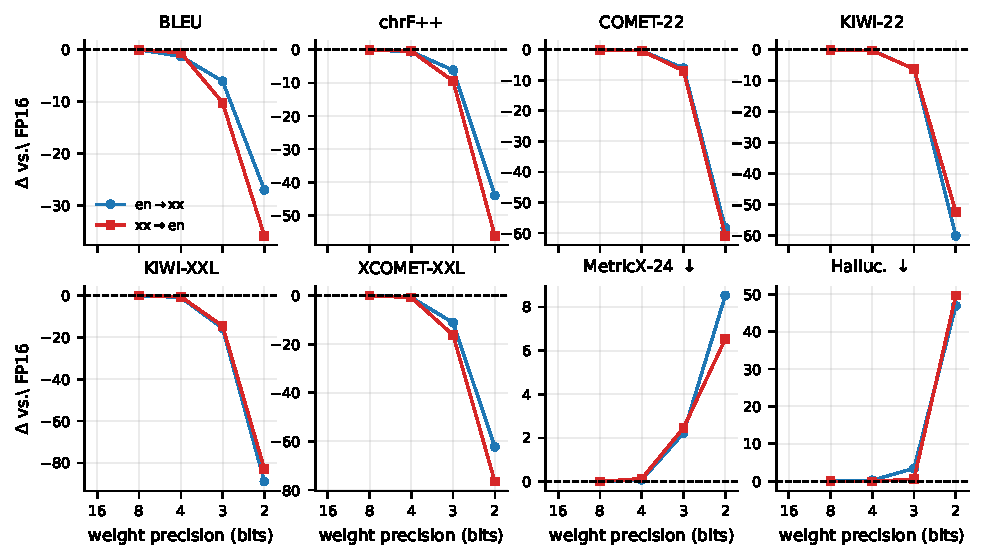
\includegraphics[width=\linewidth]{../figures/fig1_degradation.pdf}
\caption{Every metric against the FP16 beam baseline, per translation direction. The x axis is the weight precision, one tick per quantized checkpoint; the dashed line is FP16 itself, so a point below it (above, for the two marked $\downarrow$) is a loss. A precision whose run has no scores yet is simply absent from the axis.}
\label{fig:fig1_degradation}
\end{figure*}

\begin{figure*}[t]
\centering
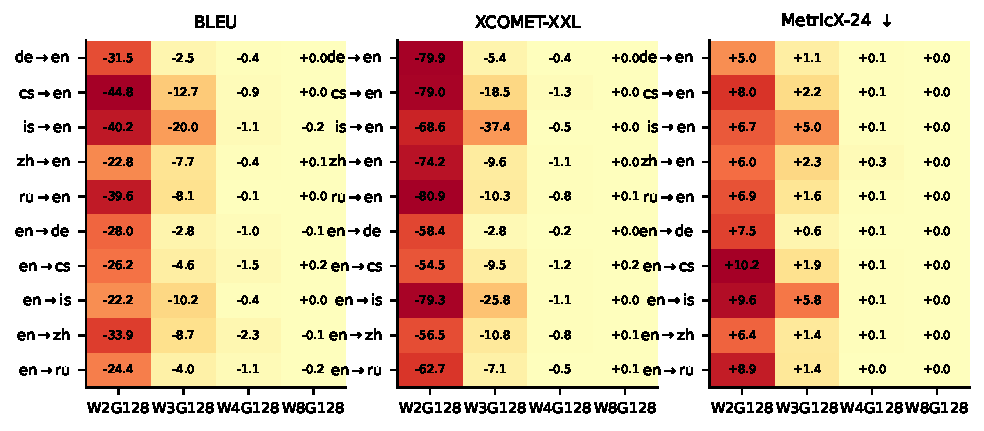
\includegraphics[width=\linewidth]{../figures/fig2_heatmap.pdf}
\caption{Difference against FP16 per direction and precision, coloured so that red is worse and green is better. MetricX-24 is sign-flipped for the colour only: the printed number is the real $\Delta$, and its sign is the opposite of the colour. Each panel is scaled to its own worst cell, so the panels are comparable in shape, not in magnitude.}
\label{fig:fig2_heatmap}
\end{figure*}

\begin{figure*}[t]
\centering
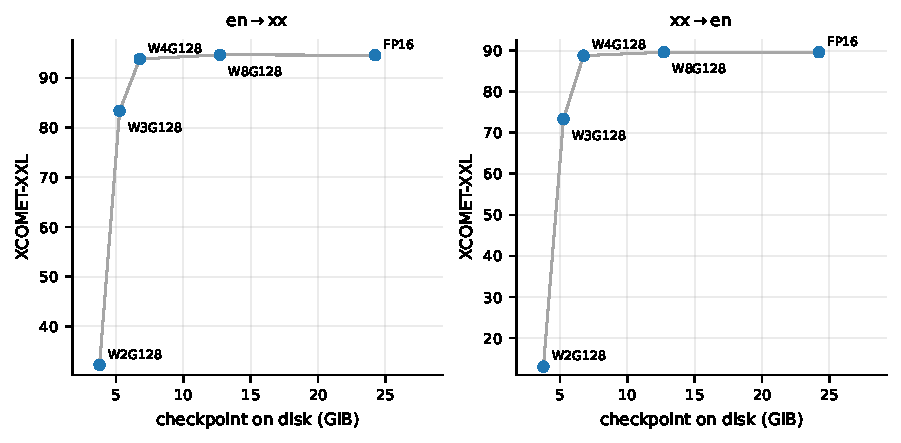
\includegraphics[width=\linewidth]{../figures/fig3_size_quality.pdf}
\caption{XCOMET-XXL against the checkpoint size on disk for both halves of the grid. The 8-bit checkpoint is 1.9$\times$ smaller and indistinguishable from FP16; 4 bits costs well under a point for another 1.9$\times$; the 3-bit step is where both the size and the score move.}
\label{fig:fig3_size_quality}
\end{figure*}

\begin{figure*}[t]
\centering
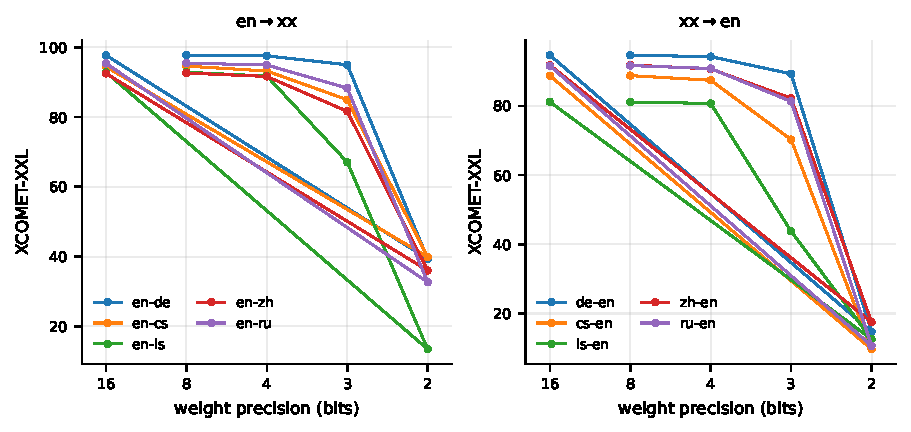
\includegraphics[width=\linewidth]{../figures/fig4_xcometxxl.pdf}
\caption{XCOMET-XXL per direction across the precision grid. All ten directions are hit, but not evenly: the low-resource ones (\texttt{is}, \texttt{zh}, \texttt{cs}) lose several times what \texttt{de} or \texttt{ru} lose at the same precision.}
\label{fig:fig4_xcometxxl}
\end{figure*}

\begin{figure*}[t]
\centering
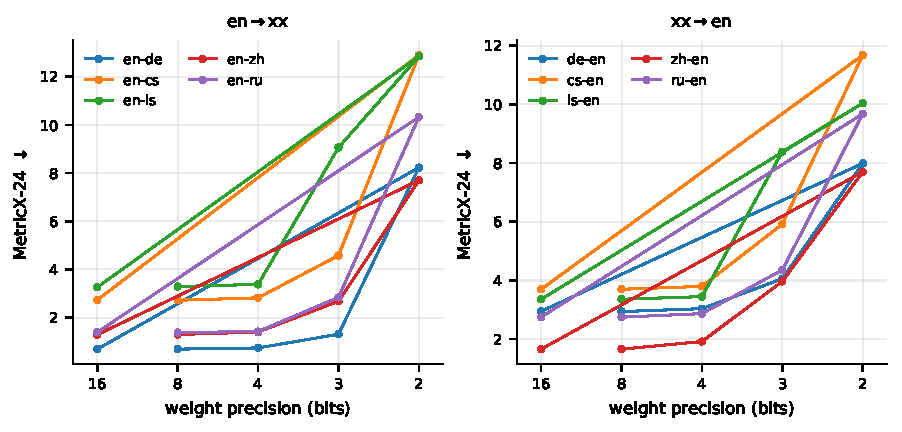
\includegraphics[width=\linewidth]{../figures/fig4_metricx24.pdf}
\caption{MetricX-24 per direction across the precision grid. All ten directions are hit, but not evenly: the low-resource ones (\texttt{is}, \texttt{zh}, \texttt{cs}) lose several times what \texttt{de} or \texttt{ru} lose at the same precision.}
\label{fig:fig4_metricx24}
\end{figure*}

\begin{figure*}[t]
\centering
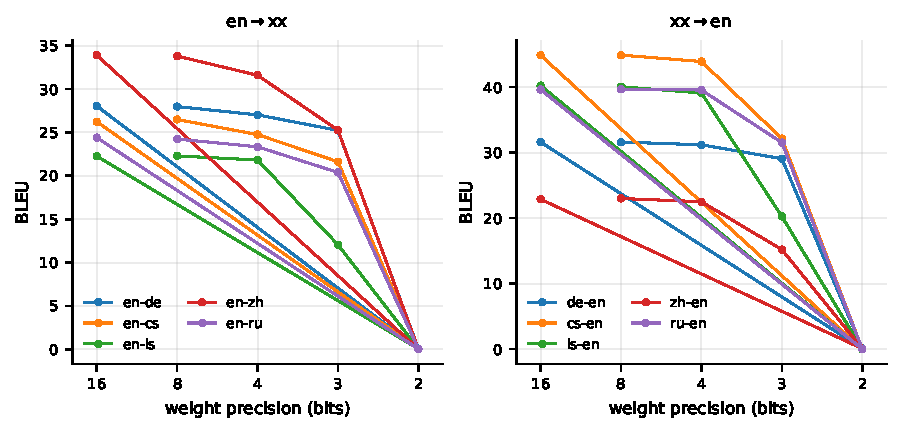
\includegraphics[width=\linewidth]{../figures/fig4_bleu.pdf}
\caption{BLEU per direction across the precision grid. All ten directions are hit, but not evenly: the low-resource ones (\texttt{is}, \texttt{zh}, \texttt{cs}) lose several times what \texttt{de} or \texttt{ru} lose at the same precision.}
\label{fig:fig4_bleu}
\end{figure*}

\begin{figure*}[t]
\centering
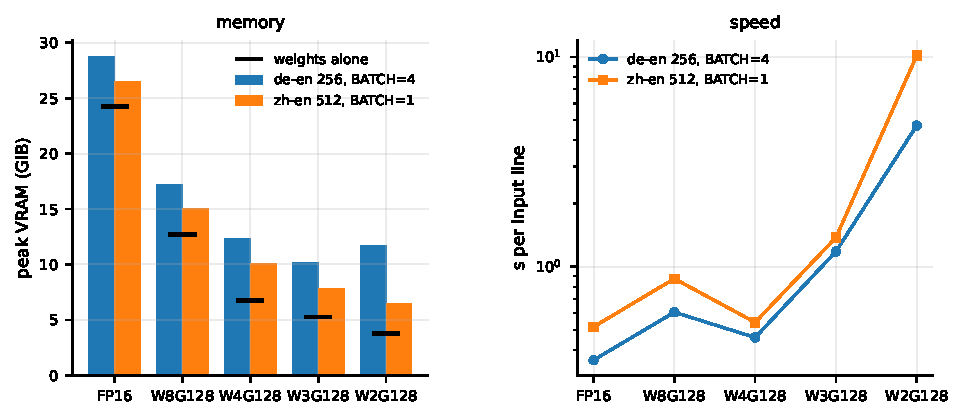
\includegraphics[width=\linewidth]{../figures/fig5_cost.pdf}
\caption{Left: the allocator peak of a timed \texttt{generate()} at the two eval protocols, with the model's own parameter footprint marked. The weights are what the compression shrinks; the rest of the bar is the KV cache and the activations, which no weight-only scheme touches, so the saving saturates well before it reaches the weights' ratio - and w2's peak rises again over w4's, because it generates 180-token outputs where w4 generates 40 and the extra KV cache outweighs the smaller weights. Right: the same checkpoints' cost per input line, log scale. The low-bit checkpoints are not cheaper per line than fp16 on this stack - GPTQModel's Triton/Torch kernels dequantize the weights and then matmul (\texttt{quant\_matmul} in \texttt{triton\_utils/dequant.py}), so every forward pays for weights it never stores - unless the batch is raised (see the batch-size section).}
\label{fig:fig5_cost}
\end{figure*}

\begin{figure*}[t]
\centering
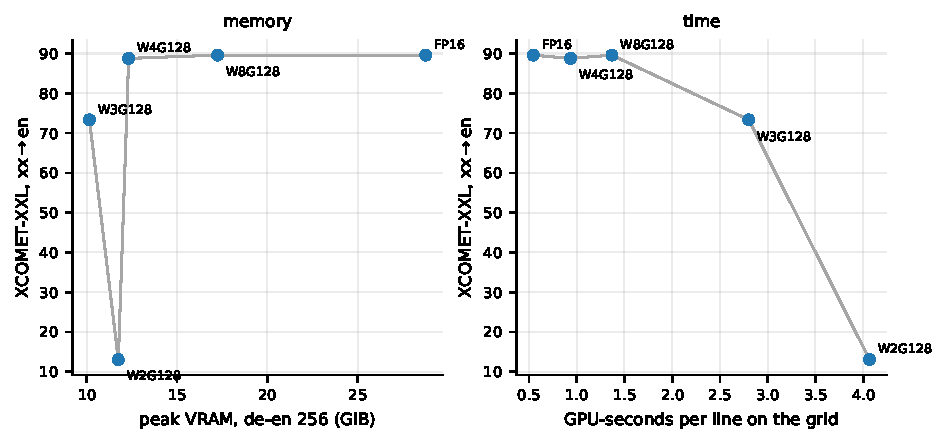
\includegraphics[width=\linewidth]{../figures/fig6_trade.pdf}
\caption{The trade the grid made. XCOMET-XXL is the harness the 3-bit collapse shows up in first (81.15 to 43.75 on \texttt{is-en}), so it is the metric that separates the two checkpoints that are worth keeping from the two that are not. Memory is the de-en \texttt{BATCH=4} peak; time is the measured grid (generation only), GPU-seconds per scored line.}
\label{fig:fig6_trade}
\end{figure*}

